\documentclass[11pt]{article}
\usepackage{amsmath}
\usepackage{tikz}
\usepackage{hyperref}

\title{A Single-File Fixture}
\author{TexCraft Test Suite}
\date{}

\begin{document}
\maketitle

\section{Introduction}
This is the first paragraph of the document. It spans several
source lines so that a single typeset line is built from material
that comes from different input lines, which is exactly the situation
that makes forward and inverse search interesting to test.

A second paragraph follows with some \emph{emphasised words}, some
\textbf{bold words} and a little bit of inline mathematics such as
$a^2 + b^2 = c^2$ or $\sum_{i=1}^{n} i = \frac{n(n+1)}{2}$, which
produces math nodes in the SyncTeX output.

\section{Display mathematics}
An equation on its own:
\begin{equation}
  \int_0^\infty e^{-x^2}\,\mathrm{d}x = \frac{\sqrt{\pi}}{2}.
  \label{eq:gauss}
\end{equation}
Equation~\eqref{eq:gauss} is followed by an aligned block:
\begin{align}
  f(x) &= (x+1)^2 \\
       &= x^2 + 2x + 1, \\
  g(x) &= \sin x \cos x.
\end{align}
Text resumes after the display.

\section{Lists}
\begin{itemize}
  \item The first item is short.
  \item The second item is a little longer and should wrap onto a
        second typeset line when the text width is not too large.
  \item Third.
\end{itemize}
\begin{enumerate}
  \item Alpha.
  \item Beta, with a nested list:
  \begin{enumerate}
    \item nested one;
    \item nested two.
  \end{enumerate}
  \item Gamma.
\end{enumerate}

\section{Floats}
Figure~\ref{fig:rule} shows a black rule, and Table~\ref{tab:numbers}
shows a small table.

\begin{figure}[ht]
  \centering
  \rule{4cm}{2cm}
  \caption{A rule standing in for a picture.}
  \label{fig:rule}
\end{figure}

\begin{table}[ht]
  \centering
  \begin{tabular}{|l|c|r|}
    \hline
    Left & Centre & Right \\
    \hline
    1 & 2 & 3 \\
    10 & 20 & 30 \\
    \hline
  \end{tabular}
  \caption{Some numbers.}
  \label{tab:numbers}
\end{table}

\section{Boxes and pictures}
Here is \fbox{a framed box}, an \mbox{unbreakable box} and a
\raisebox{1ex}{raised box} in running text.\footnote{And a footnote
that lives at the bottom of the page.}

\begin{center}
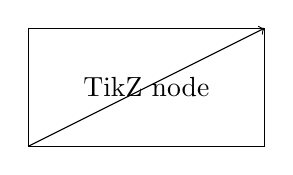
\begin{tikzpicture}
  \draw (0,0) rectangle (3,1.5);
  \node at (1.5,0.75) {TikZ node};
  \draw[->] (0,0) -- (3,1.5);
\end{tikzpicture}
\end{center}

\noindent\parbox{0.45\textwidth}{A parbox on the left with enough
text to wrap over a couple of lines.}\hfill
\parbox{0.45\textwidth}{Another parbox on the right, also wrapping
over a couple of lines.}

\subsection{More text}
The final paragraph closes the document. It has a few more words so
that it spans more than one line of output, and it ends here.

\end{document}
